\documentclass[12pt]{article}\usepackage[]{graphicx}\usepackage[]{color}
%% maxwidth is the original width if it is less than linewidth
%% otherwise use linewidth (to make sure the graphics do not exceed the margin)
\makeatletter
\def\maxwidth{ %
  \ifdim\Gin@nat@width>\linewidth
    \linewidth
  \else
    \Gin@nat@width
  \fi
}
\makeatother

\definecolor{fgcolor}{rgb}{0.345, 0.345, 0.345}
\newcommand{\hlnum}[1]{\textcolor[rgb]{0.686,0.059,0.569}{#1}}%
\newcommand{\hlstr}[1]{\textcolor[rgb]{0.192,0.494,0.8}{#1}}%
\newcommand{\hlcom}[1]{\textcolor[rgb]{0.678,0.584,0.686}{\textit{#1}}}%
\newcommand{\hlopt}[1]{\textcolor[rgb]{0,0,0}{#1}}%
\newcommand{\hlstd}[1]{\textcolor[rgb]{0.345,0.345,0.345}{#1}}%
\newcommand{\hlkwa}[1]{\textcolor[rgb]{0.161,0.373,0.58}{\textbf{#1}}}%
\newcommand{\hlkwb}[1]{\textcolor[rgb]{0.69,0.353,0.396}{#1}}%
\newcommand{\hlkwc}[1]{\textcolor[rgb]{0.333,0.667,0.333}{#1}}%
\newcommand{\hlkwd}[1]{\textcolor[rgb]{0.737,0.353,0.396}{\textbf{#1}}}%

\usepackage{framed}
\makeatletter
\newenvironment{kframe}{%
 \def\at@end@of@kframe{}%
 \ifinner\ifhmode%
  \def\at@end@of@kframe{\end{minipage}}%
  \begin{minipage}{\columnwidth}%
 \fi\fi%
 \def\FrameCommand##1{\hskip\@totalleftmargin \hskip-\fboxsep
 \colorbox{shadecolor}{##1}\hskip-\fboxsep
     % There is no \\@totalrightmargin, so:
     \hskip-\linewidth \hskip-\@totalleftmargin \hskip\columnwidth}%
 \MakeFramed {\advance\hsize-\width
   \@totalleftmargin\z@ \linewidth\hsize
   \@setminipage}}%
 {\par\unskip\endMakeFramed%
 \at@end@of@kframe}
\makeatother

\definecolor{shadecolor}{rgb}{.97, .97, .97}
\definecolor{messagecolor}{rgb}{0, 0, 0}
\definecolor{warningcolor}{rgb}{1, 0, 1}
\definecolor{errorcolor}{rgb}{1, 0, 0}
\newenvironment{knitrout}{}{} % an empty environment to be redefined in TeX

\usepackage{alltt}

\usepackage{amssymb,amsmath}
\usepackage{enumerate}
\usepackage{float}
\usepackage{verbatim}
\usepackage{setspace}
\usepackage{graphicx, multicol}

%% LaTeX margin settings:
  \setlength{\textwidth}{7.0in}
\setlength{\textheight}{9in}
\setlength{\oddsidemargin}{-.5in}
\setlength{\evensidemargin}{0in}
\setlength{\topmargin}{-1.5cm}

%% tell knitr to use smaller font for code chunks
\def\fs{\footnotesize}
\def\R{{\sf R}}
\newcommand{\bfbeta}{\mbox{\boldmath $\beta$}}
\newcommand{\bfD}{\mbox{\boldmath $D$}}
\newcommand{\bfL}{\mbox{\boldmath $L$}}
\newcommand{\bfR}{\mbox{\boldmath $R$}}
\newcommand{\bfmu}{\mbox{\boldmath $\mu$}}
\newcommand{\bfv}{\mbox{\boldmath $V$}}
\newcommand{\bfX}{\mbox{\boldmath $X$}}
\newcommand{\bfy}{\mbox{\boldmath $y$}}
\newcommand{\bfb}{\mbox{\boldmath $b$}}
\IfFileExists{upquote.sty}{\usepackage{upquote}}{}
\begin{document}


  
  
\begin{center}
\large{Bayes: Homework $10$} \\
Leslie Gains-Germain
\end{center}

\begin{doublespacing}

\begin{enumerate}

\item Here are some comments and questions. I'm not expecting you to answer these. Many of these were just ways for me to work and think through what was going on. \\

The effective number of parameters is the average deviance (found for all posterior draws of $\theta$) minus the deviance of the posterior mean of $\theta$. I'm having trouble thinking about what this quantity means, and if it's just meant to give us an idea of the posterior variance of the deviance, why is it called the effective number of parameters? Also called the bias correction for overfitting? \\

Steps for finding DIC:
\begin{enumerate}
\item Find deviance = -2*log likelihood of data given each posterior draw for $\theta$. 
\item Find the average of these deviances (deviance.avg)
\item Calculate deviance.postmean = -2log likelihood of data given the posterior mean of $\theta$.
\item Calculate pD = deviance.avg - deviance.postmean
\item Find DIC  = deviance.avg + pD
\end{enumerate}

Why is the deviance more spread out for the no pooling model? Maybe because the $\theta$'s themselves are more spread out? \\

Complete pooling model has the lowest DIC - which Gelman discusses on pages 179-180. I think this relates to something we talked about in class one day - if we used ANOVA to assess variability among groups, we would find no evidence for a difference among the group effects. \\

When would you want to use the deviance of the yreps vs the posterior predicted MSE? \\

How often is AIC actually used in a Bayesian setting? It seems like Gelman introduces it, but says it's not really applicable if we go beyond linear models with flat priors. Link and Barker talk about it being used by fields of wildlife biology and ecology fields, but I'm not sure if they mean in a Bayesian setting or not. It definitely seems easier to calculate! \\

I remember being taught in 502 that the estimate for $\theta$ is the posterior mean under squared error loss, and the estimate for $\theta$ under absolute error loss is the posterior median. Why? \\

Why do AIC, DIC, and WAIC multiply by -2? It seems like they could just be defined as the log predictive densities minus the bias correction. It seems like the -2 is a connection to the asymptotic results for likelihood ratio tests, but when comparing AICs, DICS or WAICS, is it really necessary? I guess Gelman talks a lot about putting these measurees ``on the deviance scale''. Maybe this is a silly question, I guess this is just how deviance is defined, and deviance residuals are defined this way too. \\

AIC, DIC, and WAIC focused on estimation of predictive fit, BIC (and I think Bayes Factors too) focused on estimating relative posterior probabiilities in a setting of discrete model comparison \\

Model averaging incorporates model weights in parameter estimation to account for model uncertainty. \\

Is model averaging ever used in a frequentist context? \\

Is model averaging a way to avoid choosing a model? \\

How important is model averaging? What if you use Bayesian inference but never use multimodel inference? Is that bad? \\

In some cases, it seems like model choice isn't relevant. For example, if you know the data generating process followed a binomial distribution, and you put all your prior knowledge into the model, what would you gain from comparing to other models? (maybe Gelman's point in \verb+Gelman_Rubin_discussRaftery+ paper?)

\item \begin{enumerate} 

\item I will use the analytical results derived previously in the course. For a Binomial likelihood and a $Beta(\alpha, \beta)$ prior, the posterior distribution for $\pi$ (the true probability that Liz's cupcakes taste better than Megan's) is $Beta(y + \alpha, n - y + \beta)$. So, the $Beta(0, 0)$ prior results in a $Beta(21, 7)$ posterior. The $Beta(1, 1)$ prior results in a $Beta(22, 8)$ posterior. The $Beta(2, 2)$ prior results in a $Beta(23, 9)$ posterior. I chose a $Beta(5, 2)$ for the informative prior because it gives higher density to probabilities between $0.6$ and $0.9$. I've never had Megan's cupcakes so I don't want to rule out the possibility that her's are better, but I think Liz's cupcakes would be hard to beat. Because of different tastes, however, I think there will always be some people who prefer Megan's, and this is why I have chosen a prior with lower density near $1$ (see plot below). With a $Beta(5, 2)$ prior, the posterior is $Beta(26, 9)$.

\begin{center}
\begin{knitrout}\footnotesize
\definecolor{shadecolor}{rgb}{0.969, 0.969, 0.969}\color{fgcolor}
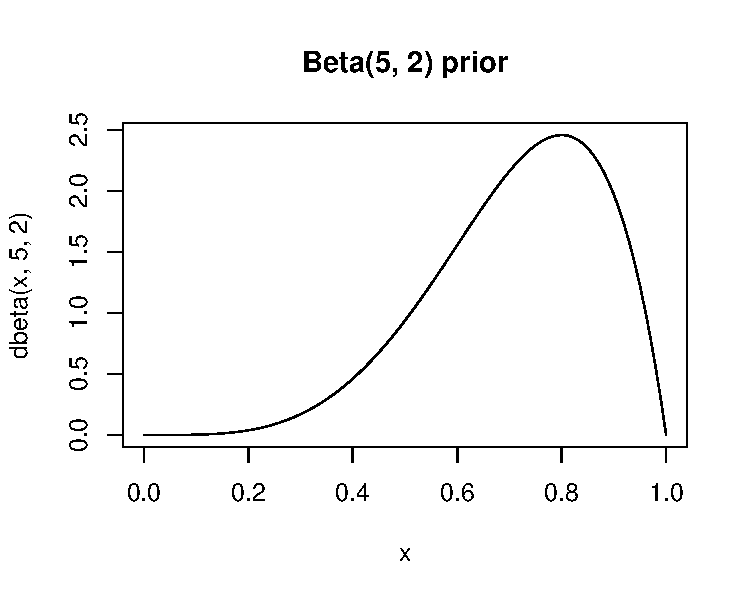
\includegraphics[width=.5\linewidth]{figure/betainform-1} 

\end{knitrout}
\end{center}

\begin{knitrout}\footnotesize
\definecolor{shadecolor}{rgb}{0.969, 0.969, 0.969}\color{fgcolor}
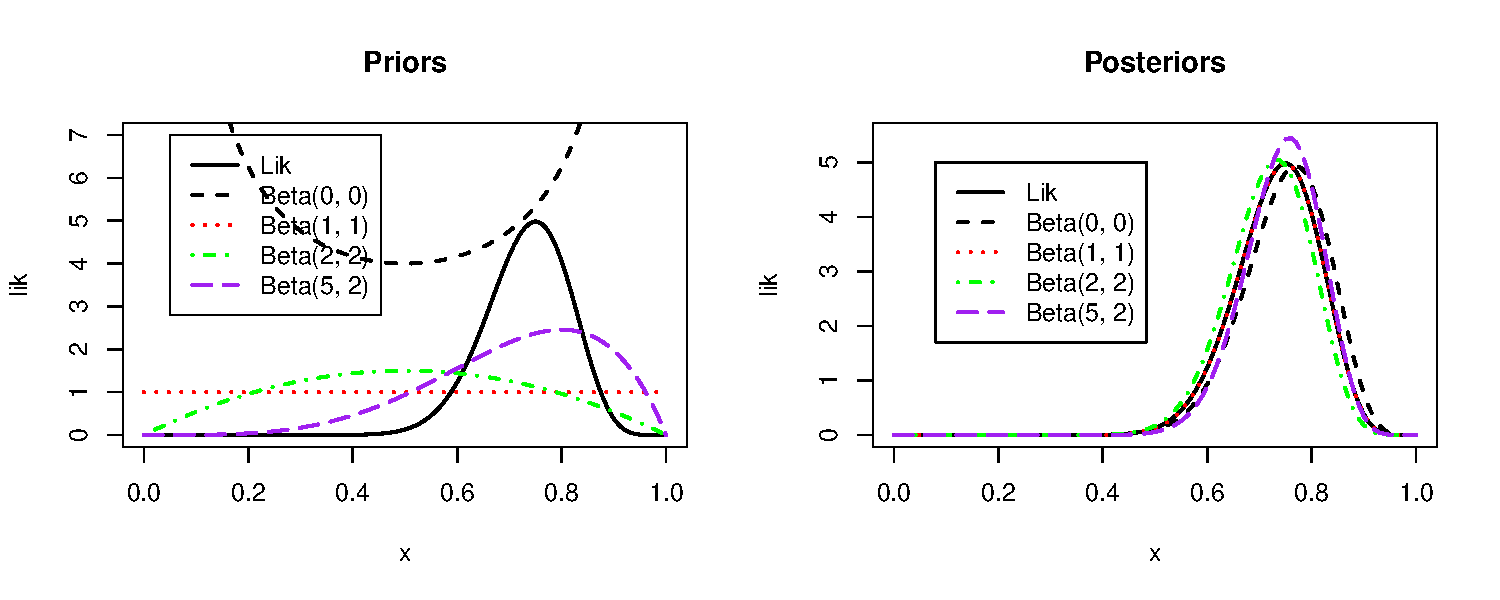
\includegraphics[width=\linewidth]{figure/plots-1} 

\end{knitrout}

When the informative $Beta(5, 2)$ prior is used, the posterior chance that the probability a Liz-made cupcake is perceived to be tastier than a Megan-made cupcake is estimated to be $0.758$ (posterior mode), with a $95\%$ posterior interval from $0.588$ to $0.871$. The posterior chance that the probability a Liz-made cupcake is perceived to be better is greater than $0.5$ is $0.998$. 

\item I show my work for finding the Bayes Factor for the $Beta(0, 0)$ prior below. I used similar calculations for the other priors.
\begin{align*}
\frac{p(M_1|y)/p(M_2|y)}{p(M_1)/p(M_2)} &= \frac{\frac{p(y|M1)p(M_1)/p(y)}{p(y|M_2)p(M_2)/p(y)}}{p(M_1)/p(M_2)} = \frac{p(y|M_1)}{p(y|M_2)} = \frac{\int_{\theta|M_1} p(y|M_1, \theta) p(\theta|M_1)}{\int_{\theta|M_2} p(y|M_2, \theta) p(\theta|M_2)} \\
&= \frac{\int_{0.7}^{1} \theta^y(1-\theta)^{28-y}\theta^{-1}(1-\theta)^{-1}d\theta}{\int_{0}^{0.7} \theta^y(1-\theta)^{28-y}\theta^{-1}(1-\theta)^{-1}d\theta} \\
&= \frac{\int_{0.7}^{1} \theta^{21-1}(1-\theta)^{7-1}}{\int_{0}^{0.7} \theta^{21-1}(1-\theta)^{7-1}} = 2.9
\end{align*}

% latex table generated in R 3.2.2 by xtable 1.7-4 package
% Sun Nov 22 19:00:30 2015
\begin{table}[ht]
\centering
\begin{tabular}{rlr}
  \hline
 & priors & BayesFactors \\ 
  \hline
1 & Beta(0, 0) & 2.90 \\ 
  2 & Beta(1, 1) & 2.11 \\ 
  3 & Beta(2, 2) & 1.59 \\ 
  4 & Beta(5, 2) & 2.74 \\ 
   \hline
\end{tabular}
\end{table}


With a $Beta(0, 0)$ prior, the bayes factor is $2.9$. Assuming neither model was favored a priori, the posterior odds that the probability a Liz-made cupcake is perceived to be tastier is greater than $0.7$ is $2.9$. In the remaining summary sentences, I assume neither model was favored a priori. With a $Beta(1, 1)$ prior, the posterior odds that the probability a Liz-made cupcake is perceived to be tastier is greater than $0.7$ is $2.1$. With a $Beta(2, 2)$ prior, the posterior odds that the probability a Liz-made cupcake is perceived to be tastier is greater than $0.7$is $1.59$. With a $Beta(5, 2)$ prior, the posterior odds that the probability a Liz-made cupcake is perceived to be tastier is greater than $0.7$ is $2.74$.

\end{enumerate}

\item Priors matter for Bayes Factors because the priors on the parameters are directly involved in the formula for a Bayes Factor $(p(\theta|M_1)$ and $p(\theta|M_2)$ in the formulas below). 
\begin{align*}
BF = \frac{p(M_1|y)/p(M_2|y)}{p(M_1)/p(M_2)} &= \frac{\frac{p(y|M1)p(M_1)/p(y)}{p(y|M_2)p(M_2)/p(y)}}{p(M_1)/p(M_2)} = \frac{p(y|M_1)}{p(y|M_2)} = \frac{\int_{\theta|M_1} p(y|M_1, \theta) p(\theta|M_1)}{\int_{\theta|M_2} p(y|M_2, \theta) p(\theta|M_2)}
\end{align*}
The prior used for $\theta$ will directly affect the value of the Bayes Factor. Bayes Factors are not always helpful when comparing models, especially when vague priors are used. Consider an example where model $1$ is $y \sim N(0,1)$, and model $2$ is $y \sim N(\mu, 1)$ with $\mu \sim N(\mu_0, \tau^2)$.
\begin{align*}
BF &= \frac{p(y|M_1)}{p(y|M_2)} = \frac{\frac{1}{\sqrt{2\pi}} e^{-y^2/2}}{\int_{\mu} \frac{1}{\sqrt{2\pi}} e^{-(y-\mu)^2/2} \frac{1}{\sqrt{2\pi\tau^2}} e^{-(\mu-\mu_0)^2/2\tau^2}d\mu}
\end{align*}

It is clear from the above equation that as $\tau$ goes to infinity, the denominator goes to $0$, and the entire equation goes to $\infty$. So, as the prior variance increases, more weight is given to the more informative $y \sim N(0, 1)$ model. So, if we chose $\tau$ to be large and used the Bayes factor blindly, we would choose the $N(0,1)$ model. If we use common sense in this situation, however, we would realize that model $2$ is the better choice. If we chose a large value of $\tau$ for model $2$ originally, then we are uncertain about the true value of $\mu$. This means that model $1$ is not a very good choice, because it reflects no uncertainty in $\mu$. Model $2$ is a much better choice because it does incorporate uncertainty in $\mu$. This example shows that Bayes Factors are not always helpful when selecting models, and trusting Bayes Factors without using common sense can be dangerous, especially when vague priors are used.

%(Side note: the $N(0,1)$ model is the more informative model because it does not incorporate any uncertainty in $\mu$).

\item A likelihood ratio is a special case of a Bayes Factor. Suppose we are testing two models, $M_1: y \sim N(0,1)$ vs $M_2: y \sim N(1,1)$. In this situation, the Bayes factor is the same as the likelihood ratio if neither model is favored a priori. It is simply a ratio of likelihood functions at $\mu = 0$ and $\mu = 1$.
\begin{align*}
BF = LR = \frac{p(y|M_1)}{p(y|M_2)} = \frac{\frac{1}{\sqrt{2\pi}}e^{-y^2/2}}{\frac{1}{\sqrt{2\pi}}e^{-(y-1)^2/2}} 
\end{align*}
I think of the Bayes Factor as being more flexible because it allows us to incorporate uncertainty in model parameters into our comparison by integrating over all values of the parameter. For an example of this, refer to the denominator of the Bayes Factor in the previous problem. Bayes Factors can also be used to compare two models of different forms, such as the poisson and geometric models in problem $5$. In a likelihood ratio test, the models being compared have to have the same form (both poisson, both binomial, etc).


\item \begin{enumerate}

\item \begin{enumerate}

\item Assuming neither model is favored a priori, the prior odds for the geometric model are $0.5/0.5 = 1$.

\item The posterior odds that the geometric model is the data generating model are $0.200$. (So the odds the poisson model is the data generating model are $5.01$). My work is shown below. 
\begin{align*}
\frac{p(M_1|y)}{p(M_2|y)} &= \frac{p(y|M_1)p(M_1)/p(y)}{p(y|M_2)p(M_2)/p(y)} = \frac{p(y|M_1)}{p(y|M_2)} \\
&= \frac{0.15^5(1-0.15)^{23}}{\frac{5^{23} e^{-25}}{1!3!5!7!7!}}
\end{align*}



\item Since the prior odds are equal, the Bayes Factor is equal to the posterior odds, $0.200$.

\end{enumerate}

\item \begin{enumerate}

\item The prior odds for the geometric model are still $1$ because neither model is favored a priori.

\item The posterior odds for the geometric model are $0.594$. My work is shown below. I recognized a beta kernel in the numerator and gamma kernel in the denominator. I show my code below for the integration. 
\begin{align*}
\frac{p(M_1|y)}{p(M_2|y)} &= \frac{p(y|M1)p(M_1)/p(y)}{p(y|M_2)p(M_2)/p(y)} = \frac{p(y|M_1)}{p(y|M_2)} \\
&= \frac{\int_{\pi|M_1} p(y|M_1, \pi) p(\pi|M_1)}{\int_{\lambda|M_2} p(y|M_2, \lambda) p(\lambda|M_2)} \\
&= \frac{\int_{1/31}^{1} \pi^5 (1-\pi)^{23} \frac{1}{30\pi^2}}{\int_{0}^{30} \frac{\lambda^{23} e^{-5\lambda}}{1!3!5!7!7!} \frac{1}{30}} \\
&= \frac{\int_{1/31}^{1} \pi^3 (1-\pi)^{23}}{\int_{0}^{30} \frac{\lambda^{23} e^{-5\lambda}}{1!3!5!7!7!}} = 0.594
\end{align*}

\begin{singlespace}
\begin{knitrout}\footnotesize
\definecolor{shadecolor}{rgb}{0.969, 0.969, 0.969}\color{fgcolor}\begin{kframe}
\begin{alltt}
\hlstd{num} \hlkwb{<-} \hlstd{(}\hlkwd{pbeta}\hlstd{(}\hlnum{1}\hlstd{,}\hlnum{4}\hlstd{,}\hlnum{24}\hlstd{)} \hlopt{-} \hlkwd{pbeta}\hlstd{(}\hlnum{1}\hlopt{/}\hlnum{31}\hlstd{,} \hlnum{4}\hlstd{,} \hlnum{24}\hlstd{))}\hlopt{*}\hlkwd{gamma}\hlstd{(}\hlnum{4}\hlstd{)}\hlopt{*}\hlkwd{gamma}\hlstd{(}\hlnum{24}\hlstd{)}\hlopt{/}\hlkwd{gamma}\hlstd{(}\hlnum{28}\hlstd{)}

\hlstd{facs} \hlkwb{<-} \hlstd{(}\hlkwd{factorial}\hlstd{(}\hlnum{3}\hlstd{)}\hlopt{*}\hlkwd{factorial}\hlstd{(}\hlnum{5}\hlstd{)}\hlopt{*}\hlkwd{factorial}\hlstd{(}\hlnum{7}\hlstd{)}\hlopt{*}\hlkwd{factorial}\hlstd{(}\hlnum{7}\hlstd{))}

\hlstd{gam} \hlkwb{<-} \hlstd{(}\hlkwd{pgamma}\hlstd{(}\hlnum{30}\hlstd{,} \hlkwc{shape} \hlstd{=} \hlnum{24}\hlstd{,} \hlkwc{scale} \hlstd{=} \hlnum{1}\hlopt{/}\hlnum{5}\hlstd{)} \hlopt{-} \hlkwd{pgamma}\hlstd{(}\hlnum{0}\hlstd{,} \hlkwc{shape} \hlstd{=} \hlnum{24}\hlstd{,} \hlkwc{scale} \hlstd{=} \hlnum{1}\hlopt{/}\hlnum{5}\hlstd{))}\hlopt{*}
  \hlkwd{gamma}\hlstd{(}\hlnum{24}\hlstd{)}\hlopt{*}\hlstd{(}\hlnum{1}\hlopt{/}\hlnum{5}\hlstd{)}\hlopt{^}\hlnum{24}
\hlstd{denom} \hlkwb{<-} \hlstd{gam}\hlopt{/}\hlstd{facs}

\hlstd{postodds2} \hlkwb{<-} \hlstd{num}\hlopt{/}\hlstd{denom}
\end{alltt}
\end{kframe}
\end{knitrout}
\end{singlespace}

\item Again, because we don't favor one model a priori, the bayes factor is the same as the posterior odds for the geometric model, $0.594$.

\end{enumerate}

\end{enumerate}

\end{enumerate}

\end{doublespacing}

\end{document}
